%!TEX root = ../dokumentation.tex
\chapter{Aufbau und Struktur des Softwaresystems}

\section{Konzept des Softwaresystems}
Für die Softwarestruktur wird ein hierarchischer Struktur nach \cite{}
In Abbildung \ref{SOF:STR} ist die Struktur und insbesondere der Datenfluss zwischen den einzelnen Modulen gezeigt.

\FloatBarrier
\begin{figure}[t]
  \centering
  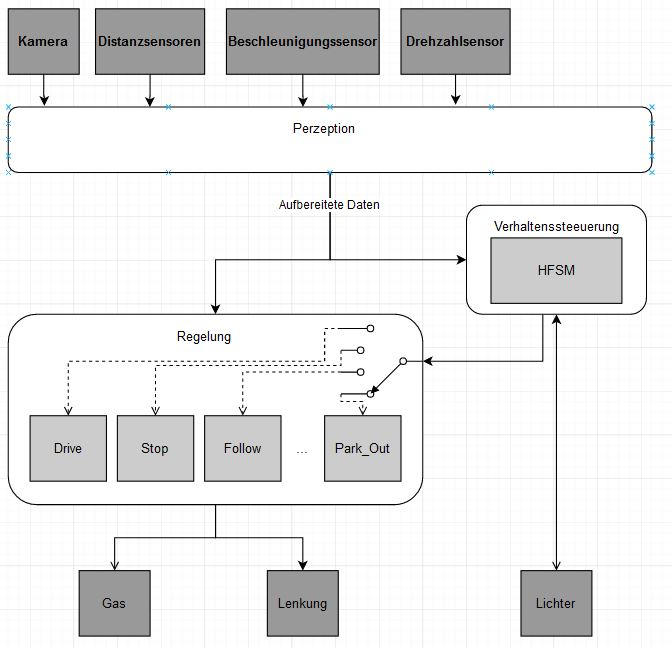
\includegraphics[width=0.5\textwidth]{images/Verhaltenssteuerung/SW_Structure.JPG}
  \caption{Softwarestruktur}
  \label{SOF:STR}
\end{figure}
\FloatBarrier

\section{Implementierung des Softwaresystems}
\subsection{Rechnersystem}

\subsection{Betriebssystem}
Für den Betrieb 
\subsection{Aufteilung der Software in Module}
\subsection{Kommunikation zwischen den Modulen}

\section{Implementierung der Verhaltenssteuerung}




\subsection{Datenaufbereitung}
Um die Daten für die Entscheidung über Zustandsübergänge zu erhalten müssen die Sensorwerte aus dem Perzeptionsmodul ausgelesen und verarbeitet werden. Dies wird in einem dafür vorgesehen Modul durchgeführt. Direkt verwendbare Daten aus dem Perzeptionsmodul werden nicht über das Datenaufbereitungsmodul an die Verhaltenssteuerung weitergegeben, sondern direkt in der Verhaltenssteuerung verwendet. In der untenstehenden sind alle Übergangsbedingungen gelistet und dargestellt ob diese im Datenaufbereitungsmodul generiert werden. 

Zeit abgelaufen         -> Datenaufbereitung
Fernbedienung aktiviert -> direkt
Taster Obstacle Evasion -> direkt
Taster Free Drive       -> direkt


\section{Grafische Oberfläche}
Die Grafische Oberfläche soll es ermöglichen währendem das Fahrzeug autonom fährt einzusehen in welchem Zustand sich das Fahrzeug befindet. Dies ermöglicht schnelle Rückschlüsse beim Testen und ermöglicht somit eine effiziente Entwicklung.
\subsection{Fahrtbeginn}
\subsection{Datenauswertung nach der Fahrt}





